\subsection{Cross Section and Luminosity}
\label{sec:WgAbout_LumiAndCS}

In this dissertation we are measuring the total cross section of the process $pp \rightarrow l \nu_l \gamma + X$ and its differential cross section in transverse momentum of the photon. A cross section in particle physics is an interaction probability per unit flux of incident particles~\cite{ref_fnal_LumiCS}. It can be interpreted as an area which must be crossed by an incident particle in order to interact with a scattering center, or, in case of a differential cross section, area $d\sigma$ within which an incident particle must appear to be scattered off by an angle $d\theta$ (Fig.~\ref{fig:CSclassical}). The relationship between $d\sigma$ and $d\theta$ gives us the expression for a differential cross section $d\sigma/d\theta$. Integrating over $d\theta$, we obtain the total cross section $\sigma$. The cross section concept illustrated in Fig.~\ref{fig:CSclassical} is generalized to be an effective area, and is generalized for two (or more) particle interactions rather than a light particle scattering off a stationary center. \\

The angle $\theta$ here is used only as an illustration of a concept of differential cross section. In particle physics we measure a differential cross section with respect to a parameter $X$ which can be a parameter of one of final state particles or of a system of final state particles. For example, a transverse momentum of a final state photon $P_T^\gamma$, an invariant mass of two final state leptons $m_{ll}$, a number of jets associated with the process $N_{jets}$ and other parameters. \\

\begin{figure}[htb]
  \begin{center}
    {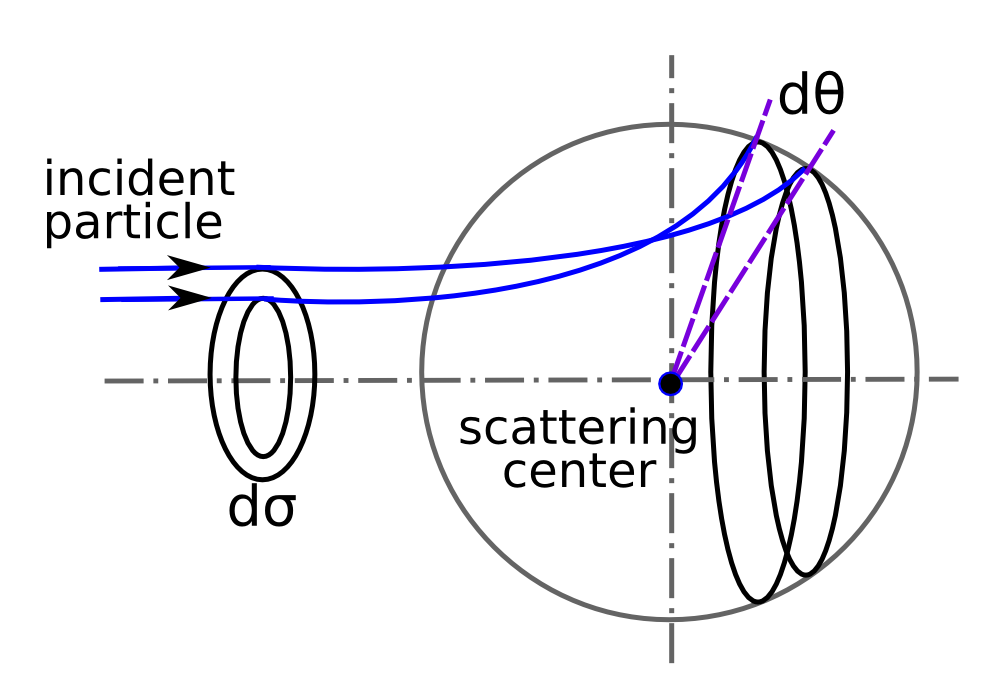
\includegraphics[width=0.70\textwidth]{../figs/WgAbout/CSclassical.png}}
    \caption{Illustration of the differential cross section concept in the classical case.}
    \label{fig:CSclassical}
  \end{center}
\end{figure}

In the scenario illustrated in Fig.~\ref{fig:CSclassical}, the number of particles passing through the area $\sigma$ per unit time is $N=L \cdot \sigma$, where $L$ is the flux of incident particles and is called luminosity. For colliding beams, the luminosity is determined by collisions frequency, the number of colliding particles in each beam, and beams cross sections. The cross section $\sigma$ of a specific process can be determined from an experiment as $\sigma=N/L$. \\

A cross section can be computed theoretically using the following expression:\\

\begin{equation}
  \sigma = \frac{W_{fi}}{F} N_{fs},
\end{equation}

\noindent{where $W_{fi}$ is a transition probability between final and initial states of the system per unit spatial volume, $F$ is the initial flux, and $N_{fs}$ is the density of final states~(\cite{ref_Halzen_Martin}, chapter~4.3). The initial flux in this expression is determined as number of incident particles per unit volume multiplied by their velocity and multiplied by number of target particles per unit volume.}\\ 

The formula of the cross section relevant for our measurement, two particles to three final state particles scattering $1+2\rightarrow 3+4+5$, is determined by the Fermi's Golden Rule~\cite{ref_Griffiths}: \\
%Further on, you do mention amplitude several times, but you never explain what it is. You may want to discuss probability amplitudes, connecting initial and final states, etc, with some basic quantum mechanics bra-ket notations, etc.
%You do not need to derive it. But you need to explain, I think, how it comes about and what it means. Just a few more sentences would be enough.

\begin{equation}\label{eq:FermiGoldenRule}
  \sigma = \frac{ 1 }{4\sqrt{(p_1p_2)^2-(m_1m_2)^2}} \int |M|^2 (2\pi)^4 \delta^4(p_1+p_2-p_3-p_4-p_5) \prod_{j=3}^{5} \frac{1}{2 \sqrt{\bar{p_j^2}+m_j^2 }}\frac{d^3\bar{p_j}}{(2\pi)^3},  
\end{equation}

\noindent{where $p_i$ are four-momenta and ${\bar{p_i}}$ are three momenta of the initial state and the final state particles, $m_i$ are masses of particles, $M$ is the process amplitude determined by the dynamics of the particles interaction. All available momenta of the final state particles is called the phase space.}\\ 
%Consider discussing parton luminosity and the cross section expression that involves the PDFs and parton-based cross sections

During proton-proton collisions, at high energy the hard scattering process occurs between partons in the protons, as discussed in Ch.~\ref{sec:Intro_ppCollisions}. Therefore, the cross section of a process $pp \rightarrow X+Y$ has two ingridients: PDFs and a partonic cross section $\sigma_{ab\rightarrow X}$. The partonic cross section is described by perturbative QCD while PDFs require non-perturbative computations and are determined, in part, from experiments (Fig.~\ref{fig:pdfs}). According to the QCD factorization theorem~\cite{ref_HardScattering}:\\
%The paragraph on the lines 473 - 478. I think you need to explain a bit more. Why can we factorize into partonic cross sections? I suggest you refer to the discussion of the proton structure in section 1.4, to the partons and parton PDFs discussed there. You also need to explain what are “i”, “j”, what are x1, x2, etc.

\begin{equation}\label{eq:ppCS_general}
  \sigma(pp \rightarrow X+Y)= \sum_{a,b} \int dx_a dx_b f_a(x_a,Q^2) f_b(x_b, Q^2) \sigma(ab \rightarrow X).
\end{equation}
%Another question I forgot to mention: in the equation 28 you have Q2. There is no integration over Q2. So what happens to it? Is it that the cross section defined by this equation a function of Q2?

In the case of $W\gamma$ process, $X$ is $l \nu \gamma$, $ab$ are $q_i \bar{q}_j$ or $q_j \bar{q}_i$. $Q^2$ is the large momentum scale that characterizes hard scattering, $f_a$ and $f_b$ are PDFs, $x_a$ and $x_b$ are fractions of momenta of the partons. In the next sections we will discuss the computation of partonic cross sections of the $W\gamma$ process and possible BSM effects.\\

